
\section[Statistics]{Statistical Interpretation of the results}\label{sect:stat}

\newcommand{\PSGcpmDo}{\ensuremath{\widetilde{\chi}_{1}^{\pm}}\xspace}


Since no excess of data over the background prediction has been observed, 
we close our study with setting upper limits on the testing signals.
This is conducted using a modified frequentist approach, namely CLs method \cite{read:CLs}.
In this method, the test statistic $q_\mu$ \cite{cowan:asymptoticCLs} is a function of the profile likelihood-ratio,

\begin{align}
q_\mu = -2 \ln \frac{\mathcal{L}(data ;\, b + \mu s)}{\mathcal{L}(data ;\, b + \hat{\mu} s)},
\end{align}

where $\hat\mu$ is the \textit{signal strength modifier} $\mu$ at the maximum point of the likelihood $\mathcal{L}$.
Then CLs is given by the following probability-ratio,

\begin{align}
CL_s = \frac{p(q_\mu \geq q_\mu^{obs} | b + \mu s )}{p(q_\mu \geq q_\mu^{obs} | b)}.
\end{align}
 
We compute CLs using a software package provided by the CMS Higgs PAG \cite{higgspag:software}.
After incorporating systematic uncertainties, an observed CLs smaller than 0.05 for a signal strength of $\mu = 1$, excludes the given signal at $95\%$ CL. Indeed, the package determines which signal strength $\mu$ excludes the testing signal at $95\%$ CL. Therefore all resulting $\mu \leq 1$ define the excluded region in the parameter space of the given signal. 


To investigate the exclusion power of our research, we study the topology of direct stau pair production and the $\PSGcpDo\PSGcmDo$ production in Simplified Models \cite{alves:sms}. 
This research deal with tau family decay of charginoes including 
$ \PSGcpmDo \rightarrow \sTau + \nu ~~\mathrm{and}~~  \PSGcpmDo \rightarrow \sNu_{\tau} + \tau $.
As discussed in Section \ref{sect:introduction}, the final state is full of $ \tau $ and $ \sTau \rightarrow \tau + \PSGczDo  $.
Hence many channels could be define, due to decays of tau to electrons, muons and hadrons.    


In this analysis, we examine the data in three different channels.
These channels include $\tau_{had}-\tau_{had}~$, $\mu-\tau_{had}~$ and $e-\tau_{had}~$.
The signal region for the $\mu-\tau_{had}~$ and $e-\tau_{had}~$ channels is defined in one bin, which is $MT2 > 90$ and $tauMT > 200$ .
Due to the sensitivity of $\tau_{had}-\tau_{had}~$ channel to the signal, we look at the data in two different bins.
The first bin is $MT2 > 90$ and the second one is $40 < MT2 < 90$ and $sumMT>250$.
We eventually combine all four bins to utilize more information from the observed and the predicted distributions.
Panels represented in Figure \ref{fig:limit_bins} show the impact of each bin on the combined result, represented by the final exclusion limit shown in Figure \ref{fig:limit_final}. The top-left panel of Figure \ref{fig:limit_bins} shows the expected exclusion region in the plane of $m_{PSGcpmDo}-m_{\PSGczDo}$
calculated by the simulated samples in the first bin of $\tau_{had}-\tau_{had}~$ channel. The top-right panel in Figure \ref{fig:limit_bins} is produced by using both bins of $\tau_{had}-\tau_{had}~$ channel.
As seen, the inclusion of bin 2 in the $\tau_{had}-\tau_{had}~$ channel causes a little expansion of the exclusion limit toward the left side (low mass 
$\PSGcpmDo$).
Two bottom panels of Figure \ref{fig:limit_bins} show the expected exclusion limit when $e-\tau_{had}~$ (left) and $\mu-\tau_{had}~$ (right) channels are included in the $\tau_{had}-\tau_{had}~$ channel.  As seen, each channel individually improves the limit on the right side of plane (high mass $\PSGcpmDo$).


%%%%%%%%%%
\begin{linenomath}
\begin{figure}[h]
\centering
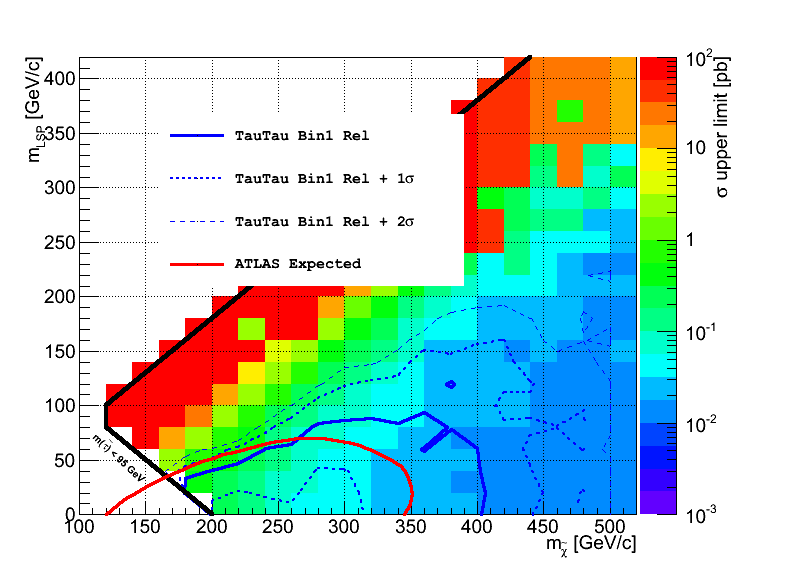
\includegraphics[width=0.49\textwidth,keepaspectratio=true]{StatisticsFig/NewFigs/TauTau_Bin1Rel.png}
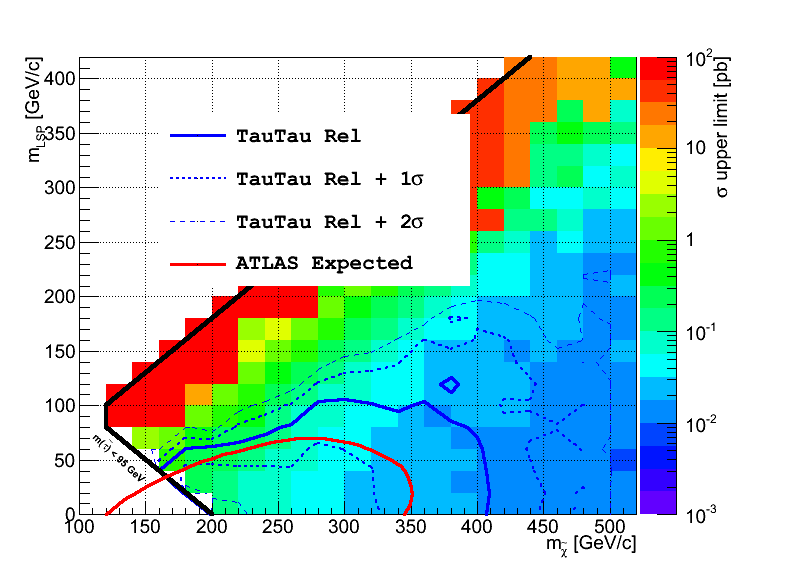
\includegraphics[width=0.49\textwidth,keepaspectratio=true]{StatisticsFig/NewFigs/TauTau_Bin1Rel_Bin2.png}
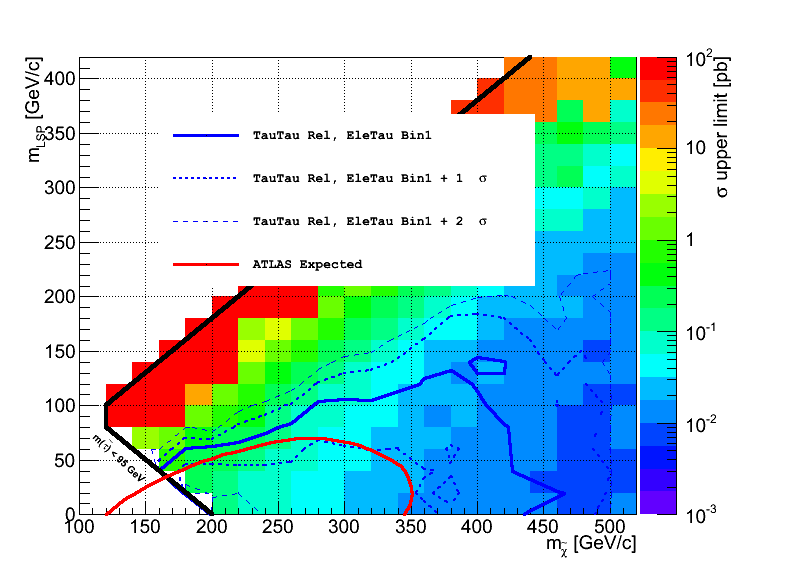
\includegraphics[width=0.49\textwidth,keepaspectratio=true]{StatisticsFig/NewFigs/TauTau_EleTauBin1.png}
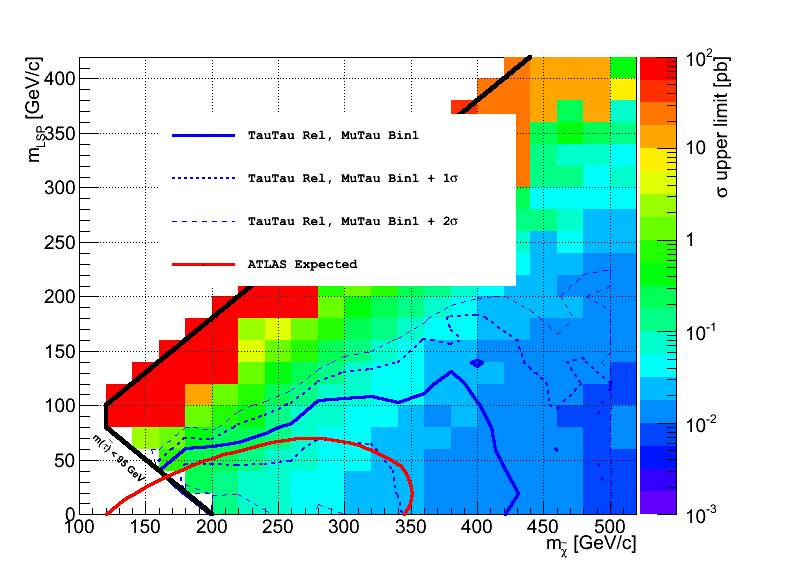
\includegraphics[width=0.49\textwidth,keepaspectratio=true]{StatisticsFig/NewFigs/TauTau_MuTauBin1.png}
\caption{These figures show the impact of each bin on the final combination. 
The top panels are related to the $\tau_{had}-\tau_{had}~$ channel including the bin 1 alone (left) and combination of bins 1 and 2 (right).
The bottom ones show the expected exclusion limit when $e-\tau_{had}~$ (left) and $\mu-\tau_{had}~$ (right) channels are included in the $\tau_{had}-\tau_{had}~$ channel.
}
\label{fig:limit_bins}
\end{figure}
\end{linenomath}
%%%%%%%%%%

Calculation of the expected exclusion limit shows that the research has potential to exclude 
%excludes 
a sizable region of the phase space, surrounded by the lines of $m_{\PSGcpmDo} = 500\GeV$ and $m_{\PSGczDo} = 150\GeV$ with an integrated luminosity of $19.6\,\fbinv$.
Figure \ref{fig:limit_final} shows the expected upper limit on the cross section of the chargino pair production in terms of Simplified Models. 
Furthermore, the figure shows the expected exclusion power considering 
$10\%$ systematic uncertainties on signal and background rates which are predicted using Monte-Carlo simulations. 
The Red curve represents the expected reach by ATLAS %\cite{cutandcountAN}
 search. As the figure shows our analysis (the blue solid curve) improves the ATLAS result in the $m_{\PSGcpmDo}-m_{\PSGczDo}$ plane.

%%%%%%%%%%
\begin{linenomath}
\begin{figure}[h]
\centering
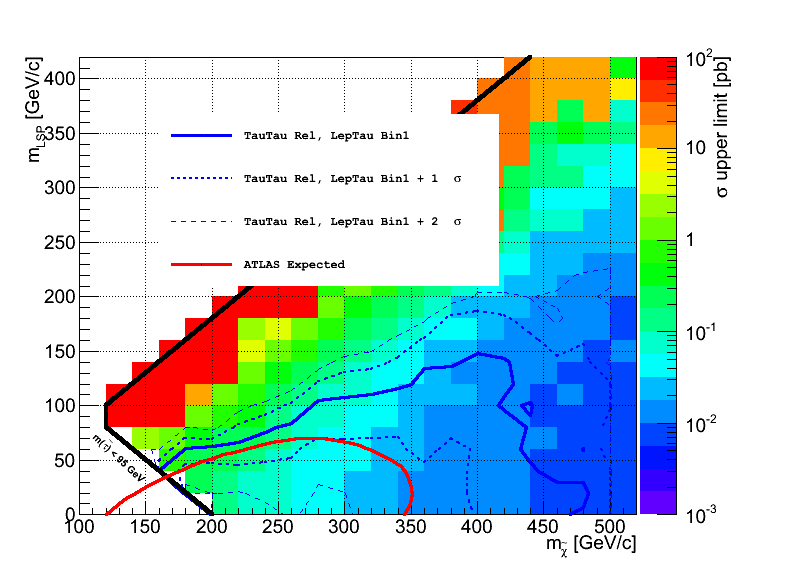
\includegraphics[width=0.7\textwidth,keepaspectratio=true]{StatisticsFig/NewFigs/Final_4BinRel.png}
\caption{Expected exclusion power in terms of Simplified Models %(T2tt-topology) 
with an integrated luminosity of $20\,\fbinv$. Backgrounds are predicted using Monte-Carlo simulations and a rough estimate of systematic uncertainties equal 
$10\%$ is taken into account.}
\label{fig:limit_final}
\end{figure}
\end{linenomath}
%%%%%%%%%%


%\rule{\textwidth}{1pt}

%In this study, we analyze data in 8 different bins (multi-bin analysis) to utilize more information from 
%the observed and the predicted distributions.
%bins' contents of the observations and the predictions.
%The bins are defined in reconstructed top quark multiplicity, zero or more. In addition, events are categorized based on the $\mttwo$ values: $125\GeV \leq \mttwo < 150\GeV,\; 150\GeV \leq \mttwo < 200\GeV,\; 200\GeV \leq \mttwo < 250\GeV,\; 250\GeV \leq \mttwo < \infty$.
%These bins are determined, for an event, based on whether the event contents reconstructed top quarks or not (2 bins) times which bin of $\mttwo$ is occupied by the event (4 bins of $125\GeV \leq \mttwo < 150\GeV,\; 150\GeV \leq \mttwo < 200\GeV,\; 200\GeV \leq \mttwo < 250\GeV,\; 250\GeV \leq \mttwo < \infty$). 

%To investigate the exclusion power of our research, we study the topology of direct stop pair production  in Simplified Models \cite{alves:sms}, with $\tilde{t}\to \PSGczDo t$ (T2tt). 
%Calculation of the expected exclusion limit shows that  
%the research has potential to exclude 
%excludes 
%a sizable region of the phase space, surrounded by the lines of $m_{\tilde{t}} = 600\GeV$ and $m_{\PSGczDo} = 175\GeV$ with an integrated luminosity of $19.6\,\fbinv$.



%Figure \ref{fig:limit_20inf} shows the expected upper limit on the cross section of the stop pair production in terms of Simplified Models. 
%Furthermore, the figure shows the expected exclusion power considering 
%$40\%$ systematic uncertainties on signal and background rates which are predicted using Monte-Carlo simulations. The black 
%dashed curve represents the expected reach by the common Cut$\&$Count \cite{cutandcountAN} search using $\MET$ trigger. 
%As the figure shows our analysis (the blue solid curve) can be comparable with other analyses and   
%it has the potential to be complementary to other analyses in some regions of the phase space.  



%%%%%%%%%%
%\begin{linenomath}
%\begin{figure}[h]
%\centering
%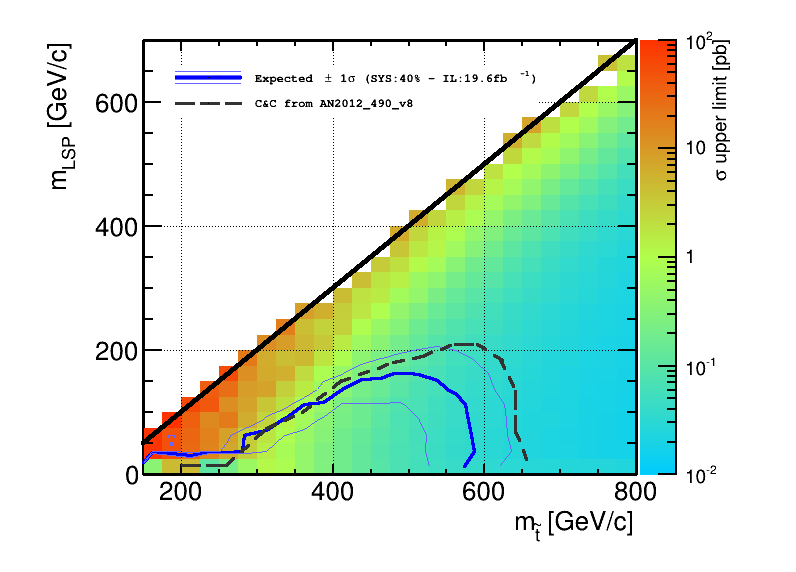
\includegraphics[width=0.9\textwidth,keepaspectratio=true]{StatisticsFig/Exc_131030_196ifb.png}
%\caption{Expected exclusion power in terms of Simplified Models (T2tt-topology) with an integrated luminosity of $20\,\fbinv$. Backgrounds are predicted using Monte-Carlo simulations and a rough estimate of systematic uncertainties equal 
%$40\%$ is taken into account.}
%\label{fig:limit_20inf}
%\end{figure}
%\end{linenomath}
%%%%%%%%%%


%%%%%%%%%%
%\begin{linenomath}
%\begin{figure}[h]
%\centering
%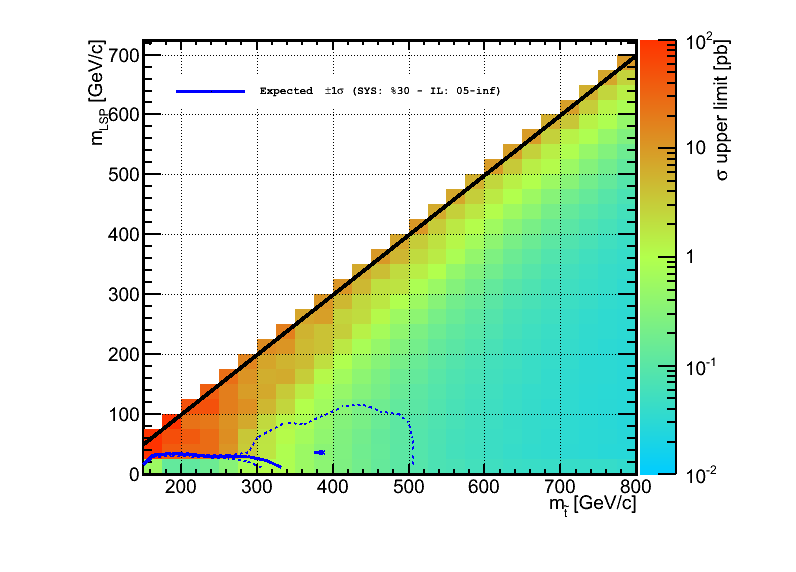
\includegraphics[width=0.7\textwidth,keepaspectratio=true]{StatisticsFig/limit_30sys_05inf_20130625.png}
%\caption{}
%\label{fig:limit_05inf}
%\end{figure}
%\end{linenomath}
%%%%%%%%%%

%%%%%%%%%%
%\begin{linenomath}
%\begin{figure}[h]
%\centering
%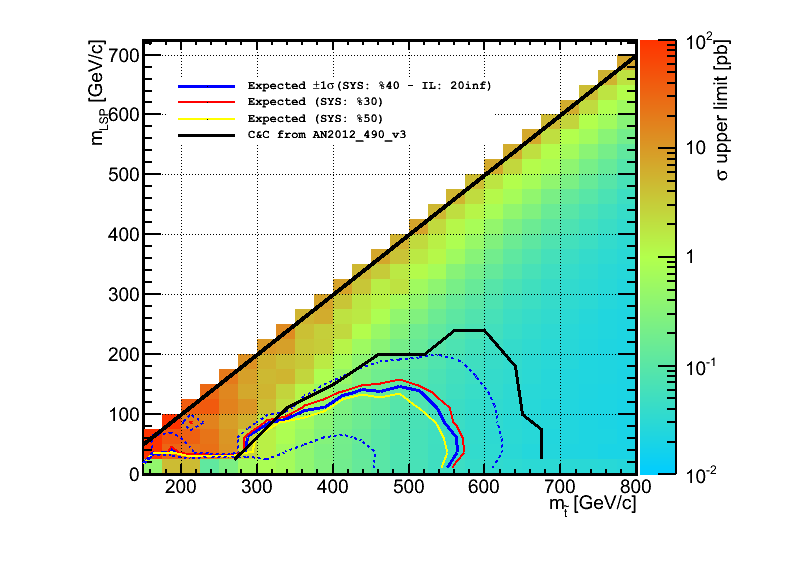
\includegraphics[width=0.7\textwidth,keepaspectratio=true]{StatisticsFig/limit_304050sys_20inf_20130625.png}
%\caption{}
%\label{fig:limit_20inf}
%\end{figure}
%\end{linenomath}
%%%%%%%%%%

